\section{Methodik}
% Einleitung
In diesem Abschnitt wird das Design des Experiments vorgestellt, sowie eine kurze Beschreibung der verwendeten Technologien und Daten.
Es wird im Detail erläutert wie das Experiment aufgebaut ist und welche Ziele damit verfolgt werden.
Die konkrete Auswertung der erhobenen Daten wird im folgenden \autoref{sec:results} vorgestellt.\\

% Datensatz
Für das Experiment liegen die von \textcolor{red}{NAME} bereitgestellten Daten vor.
Es handelt sich dabei um Artikel vom Focus-Magazin\footnote{\url{https://www.focus.de}} zum Thema Elektromobilität.
Diese Artikel wurden durch \textcolor{red}{Soziologen} aufbereitet und in die, im \autoref{subsec:economics-of-conventions} erwähnten, Welten der \ac{EC} eingeteilt.
Der Datensatz besteht aus 26 Artikeln, welche in die Welten Markt, Industrie, \textcolor{red}{TODO} und Grün unterteilt wurden.
Im Datensatz ist die Welt als \textcolor{red}{TODO} benannt, weil es in der Literatur unterschiedliche Übersetzungen und Bezeichnungen für die Welten gibt.
Zusätzlich zu der Kategorisierung in eine Welt enthält der Datensatz die Rechtfertigung bezüglich der Welt.
Diese Rechtfertigung gibt an, ob der Artikel für, gegen oder beides bezüglich einer Welt ist.
Dabei bedeutet beides nicht, dass der Artikel neutral ist, sondern dass Textabschnitte im Artikel auftauchen, welche für und gegen die Welt sprechen.\\

% Vorstudie
Es wurde ebenfalls eine qualitative Vorstudie durchgeführt, welches die Grundlage für die Masterarbeit bildet.
Diese Vorstudie wurde durch \textcolor{red}{NAME} durchgeführt und \textcolor{red}{TODO: Anhang + cite Studie}.
Zweck dieser Vorstudie war es neue Darstellungsformen der Artikel-Navigation im Online-Journalismus zu erforschen.
Unter anderem hat sich in dieser Vorstudie herausgestellt, dass die Darstellung als Begriffsverband für fünf von acht Testpersonen als informativ und interessant empfunden wurde.
Allerdings gab es auch zahlreiche Kritikpunkte am Begriffsverband in der Vorstudie.
Der Begriffsverband wies für drei Personen eine hohe Komplexität auf.
Diese sorgt dafür, dass entweder eine lange Einarbeitungszeit nötig ist oder Nutzende abgeschreckt werden.
Ebenfalls ist die Unterteilung in unterschiedliche Rechtfertigung (positiv, negativ oder beides) bezüglich einer Welt für zwei Personen eher verwirrend als sinnvoll.\\

\begin{figure}[!ht]
    \centering
    \begin{tikzpicture}
        % Erster Graph
        \begin{scope}[every node/.style={circle,thick,draw}]
            \node (A) at (0,1) {};
            \node (B) at (-2,-1) {};
            \node (C) at (2,-1) {};
            \node (D) at (0, -3) {};
        \end{scope}

        % Merkmale
        \draw (A) +(0,0.25) node[above] {Industrie};
        \draw (B) +(0,0.25) node[above, align=left] {Industrie \texttt{+}};
        \draw (C) +(0,0.25) node[above, align=left] {Industrie -};
        \draw (D) +(0,0.25) node[above, align=left] {};

        % Relationen
        \draw (A) -- (B);
        \draw (A) -- (C);
        \draw (B) -- (D);
        \draw (C) -- (D);

        % Zweiter Graph
        \begin{scope}[every node/.style={circle,thick,draw}, xshift=5cm]
            \node (A2) at (2,-1) {};
        \end{scope}

        % Merkmale
        \draw (A2) +(0,0.25) node[above] {Industrie};

        % Unsichtbare Koordinaten für den Pfeil
        \coordinate[right=1.5cm of C] (C_right);
        \coordinate[left=1.5cm of A2] (A2_left);

        % Pfeil zwischen den Graphen
        \draw[-{Stealth[length=3mm]}, thick] (C_right) -- (A2_left);
    \end{tikzpicture}
    \caption{Begriffsverband - Vorstudie (links) und vereinfachte Darstellung (rechts)}
    \label{fig:industry-comparison}
\end{figure}

% Graph
Im Rahmen der Masterarbeit wurde ein Prototyp entwickelt, welcher die Ergebnisse der Vorstudie aufgreift und weiterentwickelt.
Die hohe Komplexität wurde dadurch reduziert, dass die Anzahl der Elemente im Begriffsverband reduziert wurden.
Da für zwei Personen die Unterteilung in positiv, negativ oder beides verwirrend war, wurden diese Knoten aus dem Begriffsverband entfernt.
Dies wird in \autoref{fig:industry-comparison} beispielhaft dargestellt.
Der Knoten Industrie besitzt in der Vorstudie zwei weitere Nachfolgeknoten, welche eine positive und negative Rechtfertigung für die Welt Industrie darstellen.
Der unterste Knoten vereinigt die Eigenschaften aller darüberliegenden Knoten.
Auf diese Weise gehören Artikel, welche im untersten Knoten liegen zu der Welt Industrie und rechtfertigen sich positiv und negativ bezüglich dieser Welt.\\

\begin{figure}[!ht]
    \centering
    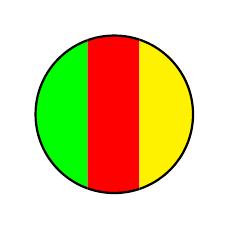
\begin{tikzpicture}
        \begin{scope}[every node/.style={circle,thick,draw}]
            \clip (-1.1,-1.1) rectangle (-0.34,1.1);
            \node[minimum size=2cm, fill=green] (A) at (0,0) {};
        \end{scope}
        \begin{scope}[every node/.style={circle,thick,draw}]
            \clip (-0.34,-1.1) rectangle (0.32,1.1);
            \node[minimum size=2cm, fill=red] (B) at (0,0) {};
        \end{scope}
        \begin{scope}[every node/.style={circle,thick,draw}]
            \clip (0.32,-1.1) rectangle (1.1,1.1);
            \node[minimum size=2cm, fill=yellow] (C) at (0,0) {};
        \end{scope}

        % \draw (A) +(0,0.25) node[above] {Industrie};
    \end{tikzpicture}
    \caption{Einfärbung des Knotens Industrie}
    \label{fig:industry-colored}
\end{figure}

% Graph kleiner, aber Infos gehen verloren
Der aus der Reduktion resultierende Graph enthält statt der vier Knoten nur noch einen Knoten.
Wenn man dies für den ganzen Graphen anwendet, dann kann der Graph \textcolor{red}{um x Knoten - nochmal nachprüfen} reduziert werden.
Der reduzierte Graph enthält jedoch auch weniger Informationen, da die Rechtfertigungen für die unterschiedlichen Welten nicht mehr dargestellt werden.
Um diesem Problem entgegenzuwirken, wurde die Repräsentation des Knotens aus \autoref{fig:industry-comparison} um drei Farben erweitert.
Diese Farben werden in \autoref{fig:industry-colored} dargestellt.
Die Farben sollen angeben, ob die Artikel sich innerhalb dieses Knotens positiv (grün), negativ (rot) oder neutral (gelb) rechtfertigen.
Diese drei Farben wurden ausgewählt, weil sie für die meisten Menschen auf dieselbe Weise emotional assoziiert werden.
So zeigen die Daten einer Studie, dass, aus der Menge der Grundfarbtöne, die Farbe Grün am positivsten und Rot am negativsten assoziiert wird \cite{color-emotion}.
Ebenfalls sind Grün und Rot Komplementärfarben, welche zwei Gegenpole darstellen sollen.
Die Farbe Gelb wird in der Studie als größtenteils positiv von Testpersonen wahrgenommen.
Gelb wurde ausgewählt, weil die Farbe Gelb bei Ampeln zum Beispiel als Zwischenzustand zwischen Rot und Grün dient.
Ebenfalls liegt Gelb im Farbspektrum zwischen Rot und Grün und ist ebenfalls ein Grundfarbton.
Auf diese Art und Weise kann möglicherweise eine Verknüpfung im Hirn für die Farbe Gelb als Zwischenzustand hergestellt werden.
An dieser Stelle sei angemerkt, dass Farben je nach Kontext unterschiedlich interpretiert werden können.
So kann die Farbe Rot, laut Studie, als warme und leidenschaftliche, aber auch als aggressive und intensive Farbe wahrgenommen werden.\\
